%!TEX root = ../template.tex
%%%%%%%%%%%%%%%%%%%%%%%%%%%%%%%%%%%%%%%%%%%%%%%%%%%%%%%%%%%%%%%%%%%%
%% chapter3.tex
%% NOVA thesis document file
%%
%% Chapter with a short laext tutorial and examples
%%%%%%%%%%%%%%%%%%%%%%%%%%%%%%%%%%%%%%%%%%%%%%%%%%%%%%%%%%%%%%%%%%%%
\chapter{Design}
\label{cha:design}

As mentioned, the main goal of this dissertation is the development of an efficient and effective query formulation visual interface. Being the first phase of solution development, the design process is where all the existing relevant problems were combined and took into account in order to explore the first solution ideas. Firstly, this chapter describes the process used to structure the problems of the current visual interface. Secondly, it is included the user and task analysis performed in order to categorize the target users in accordance with their background, expectations, and necessities. Considering the problems registered and users' necessities, the testing scenarios and the testing methodology used to evaluate the current implementation and the solution prototypes are also described. Finally, the first sketching and prototyping stages are presented in this chapter, explaining the strategies adopted to improve the user experience of the visual query builder.

\section{Problem Definition}
\label{sec:problem_definition}

The problem definition not only was the starting point for the design process but also has represented a source for the solution conception. As the actual visual interface has not been having the expected acceptability due to its interaction problems, these problems have an impactful role in the solution building process. In that way, multiple approaches were used to collect interaction problems, understanding for each of them what are the tasks involved, and the users harmed.

The following sections describe the strategies used to define the problem of the dissertation as completely as possible. The result of those analyses was combined in a table that characterizes each problem identified of the existing interface. This table is presented in \nameref{app:taxonomy_of_problems_existing_interface} and describes all the problems identified. For each problem, it was detailed the interface components involved and the Nielsen Heuristics \cite{nielsen_heuristics} affected. Moreover, the issues were classified according to the artifact and task attributes of a Framework adapted from Usability-ODC Framework \cite{in_process_usability_problem_classification_analysis_improvement}, as well as it was registered how many posts and likes have been related to the problem in the OutSystems Community \cite{outsystems_community}.

Hereinafter, the approaches and strategies used to collect and organize data regarding the existing problems of the interface will be explained. As usability issues depend on interaction with users, it is important to analyze the problems in perspective, considering in each problem the impact on users and what type of users would be most affected.

\subsection{Analysis}
\label{subsec:analysis}

The exploration and analysis of the query formulation interface was the first method used to comprehend the existing problems. The process started with the visualization of two OutSystems tutorials \cite{outsystems_tutorial_aggregates_101, outsystems_tutorial_advanced_aggregates} about visual data querying. The tutorial included also some hand-on explanations that provide an initial contextualization of the visual query builder and its functionalities. After that, other scenarios of query formulation were explored to comprehend the system barriers and difficulties.

As pointed out in \ref{sec:problem_definition}, the lack of some advanced functionalities were observed during that exploration process. However, other problems that harm the user experience and principally the efficiency and effectiveness of the user task were identified.

First of all, some functionalities were hidden, which damage the learnability of the system due to the lack of the "Recognition rather than recall" principle of the Nielsen Heuristics \cite{nielsen_heuristics}. Notwithstanding that learnability issues harm principally the novice users of all systems, there are peculiarities of this system and its environment that aggravate that problem. In that case, SQL is an alternative to perform the same tasks. Accordingly, if SQL users do not find the intended functionalities in the visual query builder due to its hiddenness, they could use SQL to perform their tasks, stopping to use the visual system.

The hidden functionalities are not only advanced features of query formulation. For instance, there is no visible option in the existing interface to add an aggregation function, such as Group By, SUM, MIN, MAX, AVERAGE, or COUNT. These options are accessible for an exclusive interaction path which requires a right-click on the column header of the attribute where the user intends to apply the aggregation function. Figure \ref{fig:rightClickGroupBy} illustrates an example of the application of an aggregation function. Other options are not always hidden but are not prepared to keep visible owing to some interface components modification. For example, despite the option to add calculated attributes is visible (after all columns of the query result table), if the query result has several columns it is necessary to scroll horizontally until the end to find that option.

\begin{figure}[htbp]
	\centering
	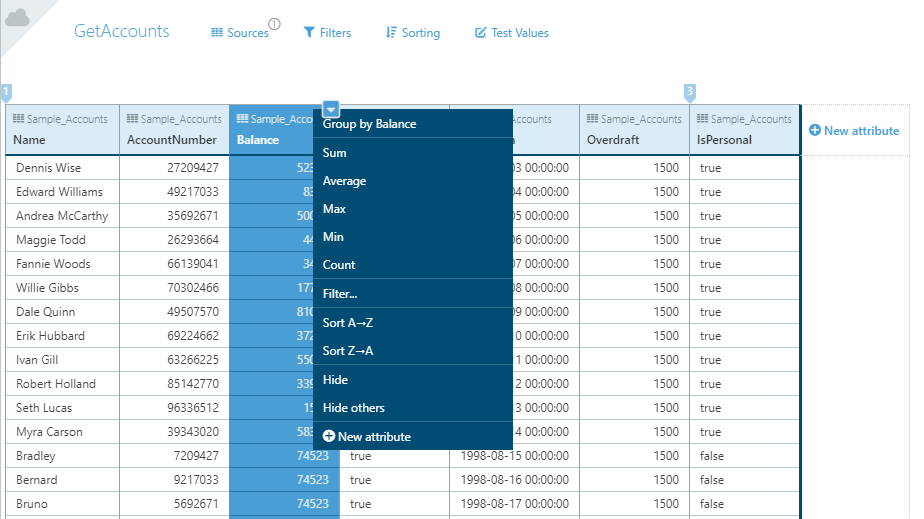
\includegraphics[height=2.5in]{right-click-group-by}
	\caption{Hidden option to add an aggregation function, since it is enclosed in a right-click on the query result table column header.}
	\label{fig:rightClickGroupBy}
\end{figure}

Furthermore, the interface has not revealed as flexible, efficient, and effective for users that need to formulate queries for professional purposes since there was identified some obstacles that prevent users from accelerating their query formulation process and reduce the rate of queries' errors. Following, there are some examples of the aspects identified through the interface's analysis, that hinder the query formulation and query comprehension, breaking the most valued proposition of the data querying visual approach:

\begin{itemize}
    \item Search engines: there is no option to efficiently search for an attribute either to look for some data in the query result or to apply some aggregation function (as illustrated in Figure \ref{fig:rightClickGroupBy}). Moreover, there is no general search in all queries, which could be useful when users need to find if some entity or variable is present in the query.
    \item Hidden columns: in the existing interface, primary and foreign keys are automatically hidden in the query result table since they were not considered as relevant data for the query output. That strategy has been implemented since the start of the interface's implementation to provide a clear output for users without a technical background, considering that they could not understand the meaning of those attributes. However, those attributes are so relevant for the query that there is a possibility to make them visible. Nevertheless, there is no efficient way to expand all hidden columns, which could difficult significantly the comprehension and formulation of all queries do not have a reduced number of entities and attributes. Figure \ref{fig:hiddenAttributes} illustrates how the hidden attributes are presented in the interface.
    \item Filter edition: In the existing interaction, the user can edit query filters using the expression editor modal, as demonstrated in Figure \ref{fig:aggregateFilterModal}. This modal is useful because it provides some guidance in the expression formulation. Thereby, users, can select the intended language expressions or the entities, attributes, or variables that need without having to recall those names. However, if users do not need that assistance, this interaction strategy could be less efficient due to the time and visual context wasted every time that a modal is opened. In that way, the modal is definitely a good feature but it should not be the only way to edit filters since it could increase the time spent to built queries. Moreover, there is no way to copy and past filter or to read effectively those content since there is no color highlighting in filters expressions.
    \item Accelerators feedback: this visual query interface has multiple accelerators that turn the query building process faster. Nevertheless, sometimes that automatic mechanisms are silent and users may not comprehend they were applied. For example, when two entities are added and have a relationship between them, the system automatically joins those entities. However, there is no highlight or other visual interaction mechanism that provides feedback to the user and shows him what action was applied.
    \item Inconsistency problems: some functionalities were accessible through a determined context and option but other alternative options do not have the same behavior;
    \item Multiple actions at once: sometimes it could be useful to do several actions at once in order to reduce the time spent to build the query. For instance, it should be possible to add multiple entities at once instead of adding one at a time; 
\end{itemize}

Those are some problems identified before communicating with users to comprehend what are the problems that harm their usage of the system every day to perform their tasks. The list of all problems identified is presented in \nameref{app:taxonomy_of_problems_existing_interface}.

In a nutshell, the first analysis and exploration of the interface lead to conclude that the interface is useful for users without technical background and has implemented good strategies that could optimize the query formulation process even more than \gls{SQL} if those strategies would be reconsidered and redesigned. Moreover, it was concluded that it is necessary to provide search engines and other accelerators to enhance the efficiency value proposition of the system. The value of the system increases if users could build queries in that system as fast as \gls{SQL} or even more.

\begin{figure}[htbp]
	\centering
	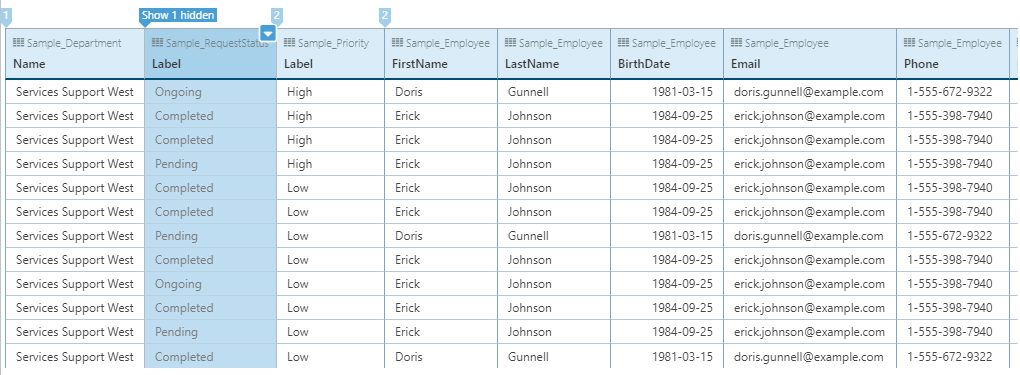
\includegraphics[height=2.0in]{hidden-attributes}
	\caption{Hidden attributes - primary and foreign keys are hidden by default.}
	\label{fig:hiddenAttributes}
\end{figure}

\begin{figure}[htbp]
	\centering
	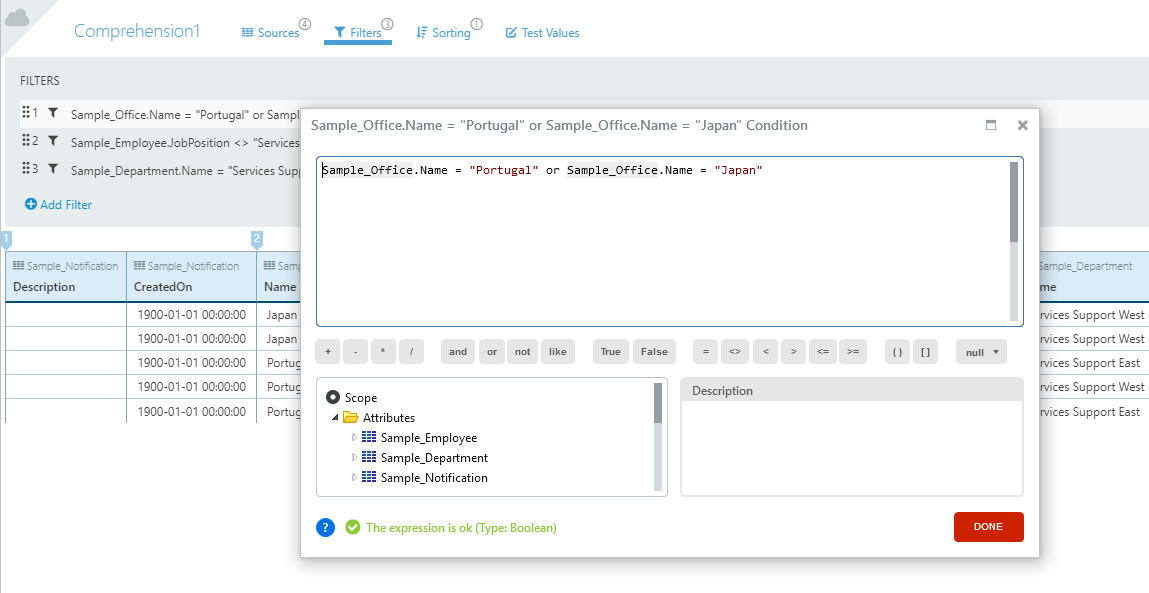
\includegraphics[height=2.5in]{aggregate-filter-modal}
	\caption{Filter edition modal - example of a filter edition after selection of the intended filter (the first one in that case).}
	\label{fig:aggregateFilterModal}
\end{figure}

\subsection{User Interviews}
\label{subsec:user_interviews}

After the analysis and study of the existing interface, there was a necessity to realize how are the usage of the visual query system for users. There was a demanding to comprehend what are the most impacting problems of the interface for users' tasks, what are the first users' reactions when asked about the utility of that interface, and if it could be applied, what are the reasons to use \gls{SQL} instead of OutSystems' visual query builder. Asking that general questions to users was the technique used to understand what is their in-depth and sincere opinion about the system utility and its most impacting problems.

Therefore, around ten user interviews were performed to explore the tool's limits and understand their impact on user actions. The interviews started with some brief questions to perceive the background of the participant. After that, more directed questions were asked in order to understand the users' opinions about the advantages and disadvantages of the visual query tool. Besides, it was asked in which situations users prefer to use \gls{SQL} instead of the visual tool. Not only was registered the situations that lead users to resort on \gls{SQL} alternative but also what are the main causes to stop using the visual query builder interface. Additionally, whenever possible, users were asked to demonstrate their problems using practical examples in order to completely understand the causes and the impact of the problems as well as other problems that have not already identified.

Furthermore, some questions about the lack of some advanced functionalities and some usability problems previously identified were prepared. The purpose of those questions is the comprehension of the user's opinion about those problems and how those problems have affected their tasks. However, it is important to understand if the user clearly identifies those problems by themselves or not. In that way, those questions only were pointed after perceiving if users would refer something about that by themselves or not. Since if they do not refer to those problems by themselves before, it is an indication that those problems have not increasingly affected them.

The results revealed that the most novice users, with less than six months of experience, consider Aggregates simple to use and it covers their necessities, referring also that it is more simple to learn than \gls{SQL}. The most experienced users, who use the OutSystems platform to develop applications, every day, for professional purposes, and have a technological background, reported that in the visual tool they cannot have a global view of the query. Moreover, they referred they work with queries that contain several tables, attributes, and business rules, and for those cases, the interface does not provide sufficient access to all functionalities.  Besides, switching between tabs in the interface to view the data sources, and the filtering and sorting criteria were other issues presented, as well as the lack of control on the query output\footnote{As referred on section \ref{subsubsec:current_progress}, when a user adds an entity to an Aggregate, all its attributes are added automatically and if the user hides them the output of the query does not change.}. Asked about the aggregation functions\footnote{Funtionality added when Simple Queries have been replaced by Aggregates (Section \ref{subsubsec:previous_work})}, they do not refer any problem with the approach interaction strategy adopted, but they have one more time referred that is so difficult to find the intended column to apply a function due to the lack of a search or navigation functionality. Finally, other usability problems that decrease the users’ satisfaction have been pointed out. such as the difficult to search something in all query or to copy and paste query components.

In conclusion, the results of this problem definition phase indicated that the interface is simple to use but could not be satisfactory for professional purpose tasks. In that way, it was pointed out the requirements to create an improved overview of the query where it is faster to comprehend what data the query is fetching as well as the implementation of interface accelerators to make the query editor powerful such as search engines and several access alternatives to the same functionality. Regardless of this, the user experience of the interface should keep simple in order to still easy to learn and easy to use for users without a superior technical background.

\subsection{Data Analysis}
\label{subsec:data_analysis}

Even though the analysis made and the first user interviews have indicated user experience problems of the interface as the factor that has been impacting the user acceptance of the visual query builder, a quantitative analysis was performed to perceive what are the operations most used by developers when they formulate queries textually. Thereby, the analysis was complemented with a metric study on queries executed on the Outsystems cloud, in order to find patterns that could justify users reasons to use \gls{SQL} instead of Aggregates. 

The queries analyzed, which have been extracted in July 2019 from customers’ projects, were built using Advanced Queries\footnote{The option of the OutSystems Platform, invoked in section \ref{subsubsec:previous_work}, that allows the query design in a textual way using a language based on \gls{SQL}.}. The data set used is composed of 214.400 statements. However, only 60.8\% were used in this study since only the queries are important for the results and not other SQL statements, such as inserts, updates, deletes, and transactions. Nevertheless, that set of 125.613 queries has duplicated results, so that these ones were removed resulting in a final data set of 67.828 queries. The operators and clauses were identified using a \gls{SQL} Parser developed in JavaScript \cite{jsSqlParser}. After obtaining the abstract syntax trees of the queries in a JSON file, that data was analyzed in a program to count the operators and the clauses that were present in the queries. 

The first measured aimed to identify the percentage of \gls{SQL} queries that contain operations not supported by the visual tool. Table \ref{tab:aggregates_operations_not_supported_stats} summarizes the number and the percentage of queries that contain these operations. It is important to refer that the intersection of the subsets is not null, so there are queries that have two or more of the indicated operations. Nevertheless, it can be observed that there was no operation that has a significant representation of the results. For example, the DISTINCT operation was the operation not supported by the visual tool with a superior percentage and it only was included in 11.78\% of the queries analyzed.

%\begin{figure}[htbp]
%	\centering
%	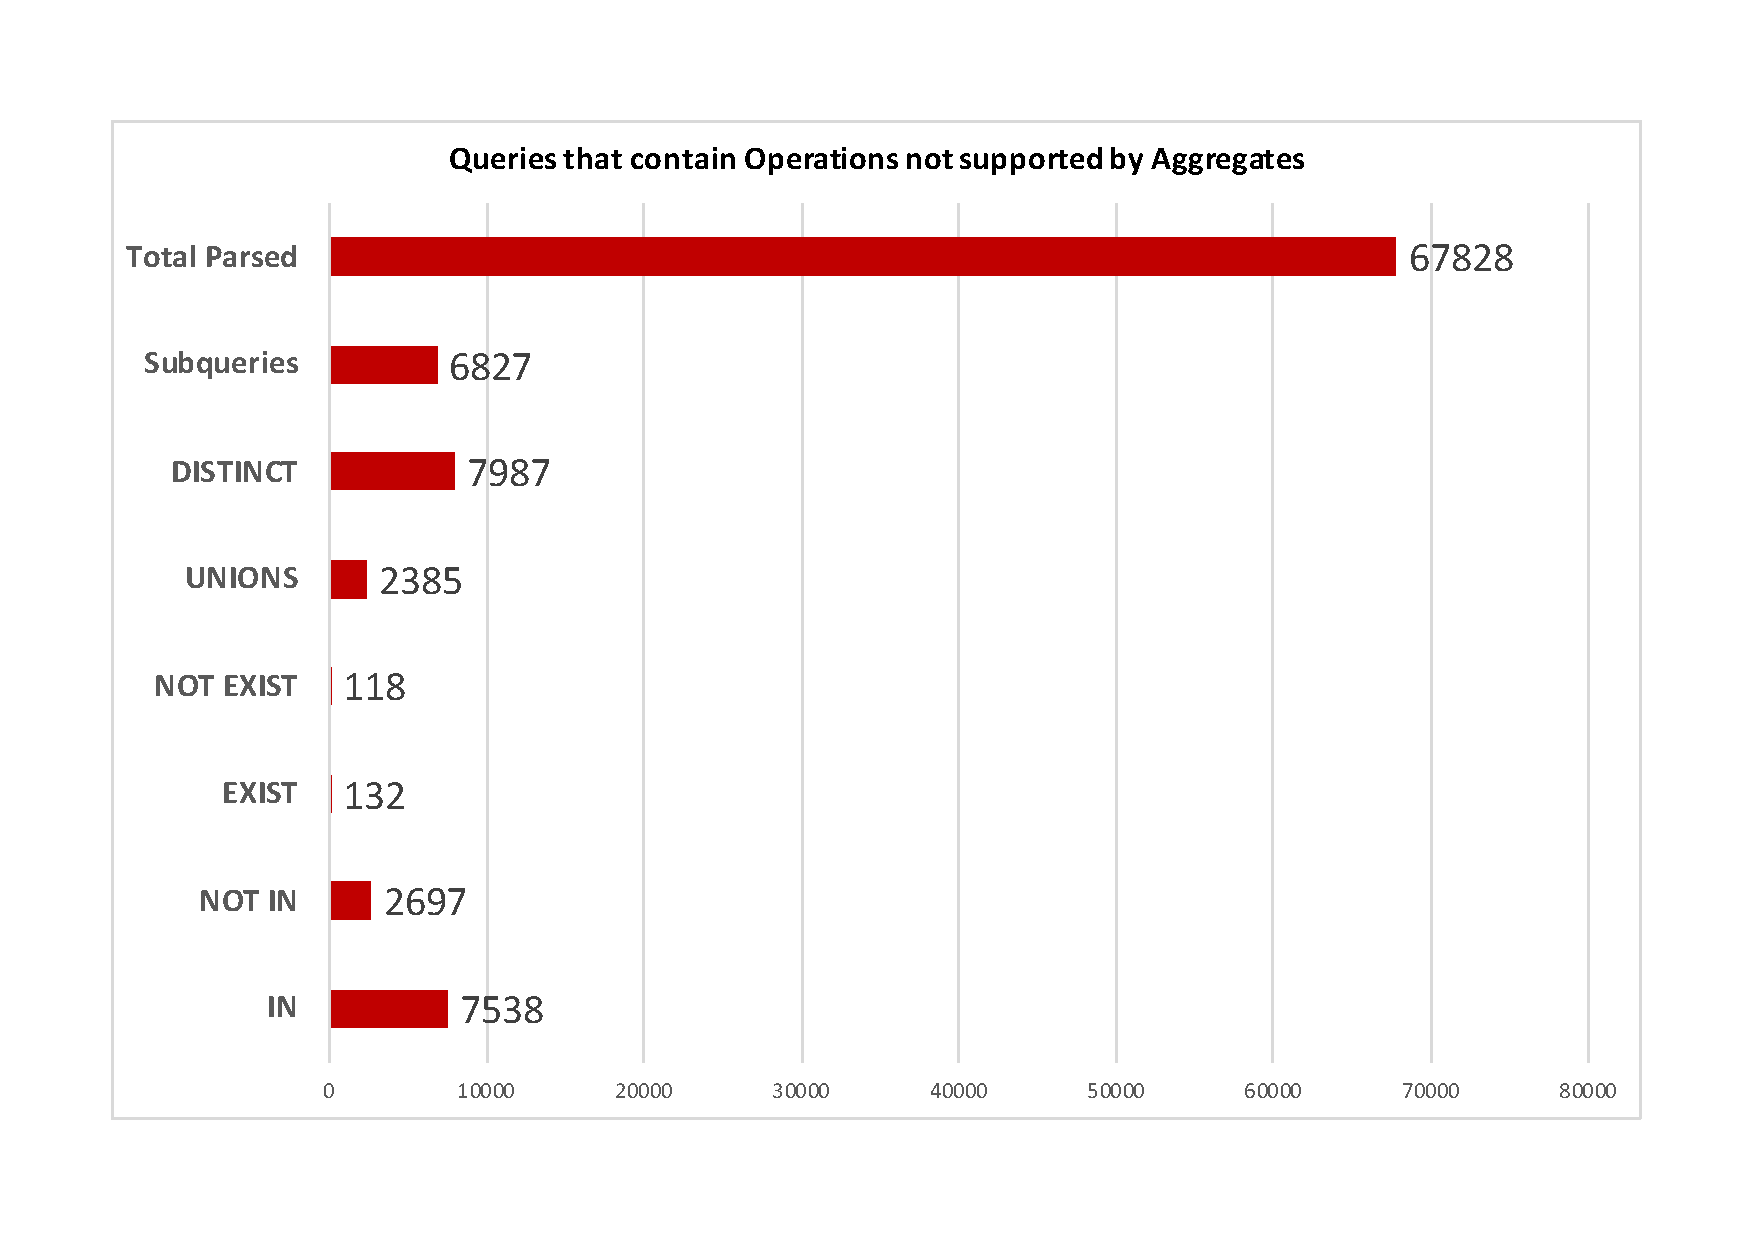
\includegraphics[height=3in]{ChartOperationsNotSupported}
%	\caption{Number of the queries that contain operations not supported by Aggregates}
%	\label{fig:aggregates_operations_not_supported_stats}
%\end{figure}

\begin{table}[tb]
	\caption{Queries that contain operations not supported by Aggregates}
	\label{tab:aggregates_operations_not_supported_stats}
\centering
\resizebox{\textwidth}{!}{
\begin{tabular}{c|c|c|c|c|c|c|c|c|}
    \cline{2-9}
    \rowcolor[HTML]{C0C0C0} 
    \cellcolor[HTML]{FFFFFF}                                 & IN      & NOT IN & EXIST  & NOT EXIST & UNIONS & DISTINCT & SUBQUERIES & Total \\ \hline
    \multicolumn{1}{|c|}{\cellcolor[HTML]{C0C0C0}Queries}    & 7538    & 2697   & 132    & 118       & 2385   & 7987     & 6827       & 67828 \\ \hline
    \multicolumn{1}{|c|}{\cellcolor[HTML]{C0C0C0}Percentage} & 11.11\% & 3.98\% & 0.19\% & 0.17\%    & 3.52\% & 11.78\%  & 10.07\%    & 100\% \\ \hline
    \end{tabular}
}
\end{table}

Furthermore, it was measured how many queries are performed using the textual language but could be designed using the visual query builder. Table \ref{tab:aggregates_supported_vs_not_supported_stats} shows the results obtained separating the queries performed in three categories:

\begin{itemize}
    \item Not Supported: Queries which include operations not supported by Aggregates, such as IN, NOT IN, EXIST, NOT EXIST, Unions, Distincts and Subqueries;
    \item Supported by Aggregates: Queries that could be designed totally using Aggregates. These are divided into two subcategories:
    \begin{itemize}
        \item Simpler: Queries which include only operations supported by aggregates excluding the indication of sorting criteria and the use of aggregation functions (e.g. GROUP BY or SUM, AVG, MIN, MAX, COUNT);
        \item More Complex: Queries that are supported by Aggregates excluding the above (simplers).
    \end{itemize}
\end{itemize}

Since user interviews suggested that aggregation functions and sorting criteria were not the main problems. The queries supported by Aggregates were divided to compare the quantitative analysis with the qualitative analysis extracted in interviews. This is important because these operations can be specified using a different interaction technique where the user changes the query when he is interacting with the query result, as mentioned in section \ref{subsubsec:current_progress}. 

\begin{table}[tb]
	\caption{Queries that could be designed using Aggregates and the queries which the tool does not support}
	\label{tab:aggregates_supported_vs_not_supported_stats}
\centering
\resizebox{\textwidth}{!}{
\begin{tabular}{c|c|c|c|c|}
    \cline{2-5}
    \rowcolor[HTML]{C0C0C0} 
    \cellcolor[HTML]{FFFFFF}                                 & Not Supported & Supported (Simpler) & Supported (More Complex) & Total \\ \hline
    \multicolumn{1}{|c|}{\cellcolor[HTML]{C0C0C0}Queries}    & 28130         & 24026               & 15672                    & 67828 \\ \hline
    \multicolumn{1}{|c|}{\cellcolor[HTML]{C0C0C0}Percentage} & 41.5\%        & 35.4\%              & 23.1\%                   & 100\% \\ \hline
    \end{tabular}
    }
\end{table}

In the set of queries analyzed, around 58.5\% could be designed using Aggregates, is evident that the lack of support of some \gls{SQL} expressions might not be the main problem. Under the circumstances, the results were discussed together with the stakeholders. It was determined that the main problem was the usability of the system. 

In conclusion, the results of the quantitative analysis have confirmed the assumptions pointed out after the analysis and exploration of the interface and the first user interviews. All the studies made have concluded that the main priority of the project should be the usability improvement of the visual querying tool interface. Thereby, there are metrics that sustain the conclusions made in the problem definition phase.

\subsection{Community Ideas}
\label{subsec:community_ideas}

Since OutSystems has a wide a worldwide Community of developers and they can use the OutSystems Community Website \cite{outsystems_community} to express their problems or difficulties or even new contribution ideas for the product, it was thought that could be advantageous for the final solution if ideas and problems of community ideas would be taken into account. Accordingly, all 306 posts of category "Aggregates \& Queries" were analyzed in order to extract useful information for the design phase of this dissertation.

First of all, it has been taken into account for each post if the topic is related to the lack of some functionalities or related to some problems in the interface. That approach leads to perceive that the predominance of the posts are about usability problems of the interface, whereas there are a reduce quantity of posts about functionalities not supported.

Therefore, the users’ problems and suggestions regarding usability problems or enhancements of the interface were processed to transform that information as a relevant input to the next design phases. Despite all the problems and suggestions identified are detailed in \nameref{app:taxonomy_of_problems_existing_interface}, following there are some examples of the problems and suggestions  indicated in the OutSystems Community:

\begin{itemize}
    \item Search engines: users requested in multiple posts alternatives to search for an entity, attribute, or filter inside the query. Not only they refer that the readability in the interface is difficult since there is no color highlight in the text but also there is no possibility to search for the intended fields. Also, they refer that is extremely important for their work since they need to build queries with a large set of entities, attributes, and conditions;
    \item Filters Edition: it was pointed out in several posts suggestions to improve interface in order to support filters comments with color highlighting, since they could be useful to explain the intention of the filter, or even the possibility to disable filters instead of deleting them.  
    \item Result Count: there is no visible count of how many rows the query result has;
    \item Accelerators and Utilities: regarding this, it has been suggested different accelerators in order to accelerate and streamline the query formulation process as well as different ways to present the query structure since in the user's point of view the query readability provided with the existing interface should be improved.
\end{itemize}

In summary, beyond the necessity of new advanced functionalities, the developers on the OutSystems Community have indicated different situations where the interface turns out not to be as powerful as it could be, since there is a lack of utilities or accelerators that could assist users keeping his task on track.

\subsection{Current Implementation Evaluation}
\label{sec:current_implementation_evaluation}

In order to analyze users' behavior while they are interacting with the visual query interface, it was prepared testing scenarios used to evaluate usability attributes of the interface.\footnote{This evaluation process is described in sections \ref{subsec:testing_scenarios} and \ref{subsec:evaluation_technique}.} The main purpose of this evaluation is the analysis of the current effectiveness, efficiency, and learnability of the system to compare them, on the final of this dissertation, with those of the proposed solution. 

Nevertheless, during the tests, users have mentioned other details of the interface that could be a useful input for the next design iterations. In that way, that feedback was also taken into account and registered as all the other issues identified. Thereby, \nameref{app:taxonomy_of_problems_existing_interface} includes also all problems or possible enhancements identified during the user testing process of the existing visual query interface.


\section{User and Task Analysis}
\label{sec:user_and_task_analysis}

After obtaining a detailed and wide view of the existing problems, the following step was the exploration of how those problems can be solved. As the main goal is the development of an improved interface that gives to the users a solution to manage data queries efficiently, and effectively through intuitive interaction strategies, users are a crucial factor that must be taken into account throughout the entire solution development. Each user has his peculiarities, then the user experience of the solution should be adapted as much as possible to the target users of the query formulation system.

\subsection{User Groups}
\label{subsec:user_groups}

Considering that users will only use the visual query system if they use the OutSystems Platform, that low-code development context where the query system is inserted cannot be dissociated from the user analysis. Thereby, the user analysis process started by a study to categorize the profile of OutSystems Platform users according to the specificities of the data querying domain.

Since the low-code development paradigm has integrated more people who do not has the strict software engineer profile into software development tasks, the users of the OutSystems Platform do not have the same backgrounds, requirements, and expectations. If, on the one hand, there are OutSystems Developers that have Computer Science academic backgrounds or similar, and experience working with low-level programing language, on the other hand, there are business experts or specialized in other engineering fields that are also developing in OutSystems. In that way, the provided query building experience should be a hybrid approach that covers the traditional software developers demands without turning the development and the language intuitive for people that are not familiarized with classical development patterns, terminologies, or processes.

As the set of users that may use the visual query system is so broad and heterogeneous, it was necessary to analyze and register the aspects of the user profile which could branch out their needs and expectations in different directions. In this sense, the following three points of the users' background were considered the ones that could accurately cluster the users' expectations and demands, considering the usage context of the interface, which combines software development, low-code development, and relational databases querying domains:


%Key Points:
%--Computer Science Background
%-
%-
%-
%--OutSystems Development Experience
%-
%-
%-
%--Data Tools Expertise
%-
%-
%-

\begin{itemize}
    \item \textbf{Computer Science Background:}
    \item \textbf{OutSystems Development Experience:}
    \item \textbf{Data Tools Expertise: }
\end{itemize}


\begin{table}[h]
    \caption{User Groups}
    \label{tab:user-groups}
    \begin{tabular}{|
    >{\columncolor[HTML]{C0C0C0}} m{3cm} |m{12cm}|}
    \hline
    \begin{tabular}[c]{@{}l@{}}Software \\ Developer\end{tabular}   & Software Developer or Engineer who has a good and solid previous knowledge of programming and databases. The principal capabilities of these users are programming languages, such as C\#, SQL, and others. These users cannot abstract their previous knowledge, so communication with these users is more technical and specific. Finally, this user group is not an expert in low-code development. However, as they have solid programming, logic, and database knowledge, probably these users could develop some applications using low-code. \\ \hline
    \begin{tabular}[c]{@{}l@{}}OutSystems \\ Developer\end{tabular} & Independently of their background, these users are experienced in OutSystems. That way, whether or not you know all the basic knowledge, they are proficient and faster in low-code development. This is your principal characteristic that should be taken into account. \\ \hline
    \begin{tabular}[c]{@{}l@{}}Citizen \\ Developer\end{tabular}    & Users who do not have an extensive programming or software development background, since that is not their main area. Although they could develop some apps outside software development units, this is not their specialty. As some of these users may not know how relational databases work, they may use other applications, such as Microsoft Excel, Google Sheets, Salesforce, and others to manage data. \\ \hline
    \end{tabular}
    \end{table}

\subsection{Testing Scenarios}
\label{subsec:testing_scenarios}

\subsection{Evaluation Technique}
\label{subsec:evaluation_technique}

\section{Sketching and Prototyping}
\label{sec:sketching_and_prototyping}

\subsection{Sketching}
\label{subsec:sketching}

\subsection{Paper Prototype}
\label{subsec:paper_prototype}
% Do not forget to refer that due to COVID-19 the Paper Prototype was scanned and mounted as a low-fidelity prototype using InVision App.

\subsubsection{Design}
\label{subsubsec:paper_prototype_design}

\subsubsection{Implementation}
\label{subsubsec:paper_prototype_implementation}
% It is important to refer the implementation complexity of the prototype in InVision due to the interface complexity.

\subsubsection{Evaluation}
\label{subsubsec:paper_prototype_evaluation}
%Comparison with Current Implementation Evaluation



\clearpage


\section{Proposed Implementation}
\label{sec:proposed_implementation}
According to the analysis made and the results concluded, the implementation covers an iterative design process aiming at improving the usability of Aggregates, the component of the OutSystems Platform to visually build queries. The prioritized improvements of the \gls{VQL} expressiveness (IN / NOT IN and DISTINCT) will be included in the project, if possible, depending on the development progress of the usability issues. If in the next stages of development it is found that it is possible to address these expressiveness problems without impairing the development related to improving usability, these will be designed and developed, otherwise, the focus will be only the usability improvement. %TODO: Falta explicar melhor em que consiste melhorar a usabilidade, resumindo quais sao os problemas

As mentioned above in Section \ref{subsubsec:current_progress}, the actual visual tool include in the interface sections to design queries visually and to view their results. Therefore, the aim is to design and evaluate how these two parts of the interface can be changed to improve the usability of the system. In a nutshell, there are two aspects that are needed to be taken into account, in order to guide the design process: the simplicity, efficiency and effectiveness to construct queries independently of how many tables or conditions, and the readability of the global query to perceive what data of the database the query will be gathering.

%Never forgetting these guidelines, the query parts specified in Table X will guide the design process, studying and evaluating solutions to improve the specification method, without harming the query overview readability and the interaction strategies to specify the other parts of the query. 

The design and development process shall be divided into an initial preparation and analysis phase and the iterative design process phase:

\begin{itemize}
    \item \textbf{Preparation and analysis phase}: before the development of the prototypes, the users and the tasks of the should be analyzed. Also, it should be started sketching as a means to bring up ideas that could represent starting points to tackle the existing problems. Therefore, this preparation process before the development of the prototypes will include the following tasks:
    \begin{itemize}
        \item \textbf{Data Extraction}: although there are results obtained in the interviews and in the quantitative analysis process, detailed in \ref{sec:requirements_analysis}, additional data about the queries design using aggregates also will be extracted. It could be important to the process to understand the user's usage of the existing visual tool since the results obtained are only about the queries built using the textual language;
        \item \textbf{User and Task Analysis}: users and their tasks will be characterized and classified regarding the concepts presented in section \ref{subsubsec:user_and_task_analysis} This description and classification will be used not only as a reference point throughout the design process but also to define the most important trade-offs on usability attributes;
        \item \textbf{Sketching}: the phase where the first sketches of possible solutions will be designed. The most important is the initial exploration of several possibilities to tackle the problems through a low-level and fast approach. As referred in section \ref{subsubsec:sketching_and_prototyping} it is useful to discover new ideas, keeping register the first approaches to tackle the problems. At the later phases, the sketches could be useful to remember the starting point of the design process;
    \end{itemize}
    \item \textbf{Iterative design}: this process starts with low-level prototypes and in each iteration, these are evaluated to create higher fidelity prototypes in the next iteration. However, as referred in section \ref{subsubsec:sketching_and_prototyping}, there are different strategies to reuse or not the prototypes over iterations. In this project, an evolutionary strategy where the prototypes developed are used as the basis for the next design iteration will be adopted. Moreover, the design process will include three iterations:
    \begin{itemize}
        \item \textbf{Paper Prototype (1st iteration)}: regarding the information obtained in user and task analysis, and the main ideas raised on the sketching stage, a first functional paper prototype will be built. The evaluation of the entire concept of the first interaction strategies is the main concern of this phase. Cognitive Walkthrough and Observational Methods of user testing will be the evaluation techniques used on this phase;
        \item \textbf{Low-fidelity Prototype (2nd iteration)}: using the results of the previous iteration, the idea is to develop a low-fidelity computer prototype on technologies, such as Balsamiq \cite{balsamiq} or Mockingbird \cite{mockingbird}, which although do not create native applications, allow the employment of visual components and animations more similar with the intended in the final solution. So, more aspects can be tested regarding a higher complexity and fidelity of the interface. At this stage, Heuristic Evaluation will be used by experts and more user tests will be performed. However, it is likely that not only Observational Methods are performed. Experimental Methods could be necessary to test specific hypotheses or discuss what is the better option between a set of possible implementations. Moreover, Query Methods, like questionnaires, could be valuable as well, to understand the user’s satisfaction;
        \item \textbf{Final Prototype (3rd iteration)}: computer prototype integrated in the OutSystems Platform. The development focuses on the presentation layer of the application due to improving the Aggregates interface and \gls{UX}, using the new results obtained. The front-end of the application is developed in React \cite{react}, using the TypeScript \cite{typescript} language. Accordingly, these are the technologies that will be used in the development of the final prototype. Being the last prototype and consequently the final result of this project, it will be evaluated also by users and experts to summarize the final results of all the design and development process;
    \end{itemize}

\end{itemize}

\section{Work Plan}
\label{sec:work_plan}
According to the proposed implementation approach, Figure \ref{fig:work_plan} represents a work plan until the final of the thesis, scheduling each one of the tasks explained in the previous section throughout the remaining weeks. The tasks are assigned to its respective major phases, and the focus on the writing of the document is primarily at the end of each phase or iteration to summarize all the contents addressed during these periods, although the report can be updated every time it reveals useful.

\begin{figure}[hb]
	\centering
	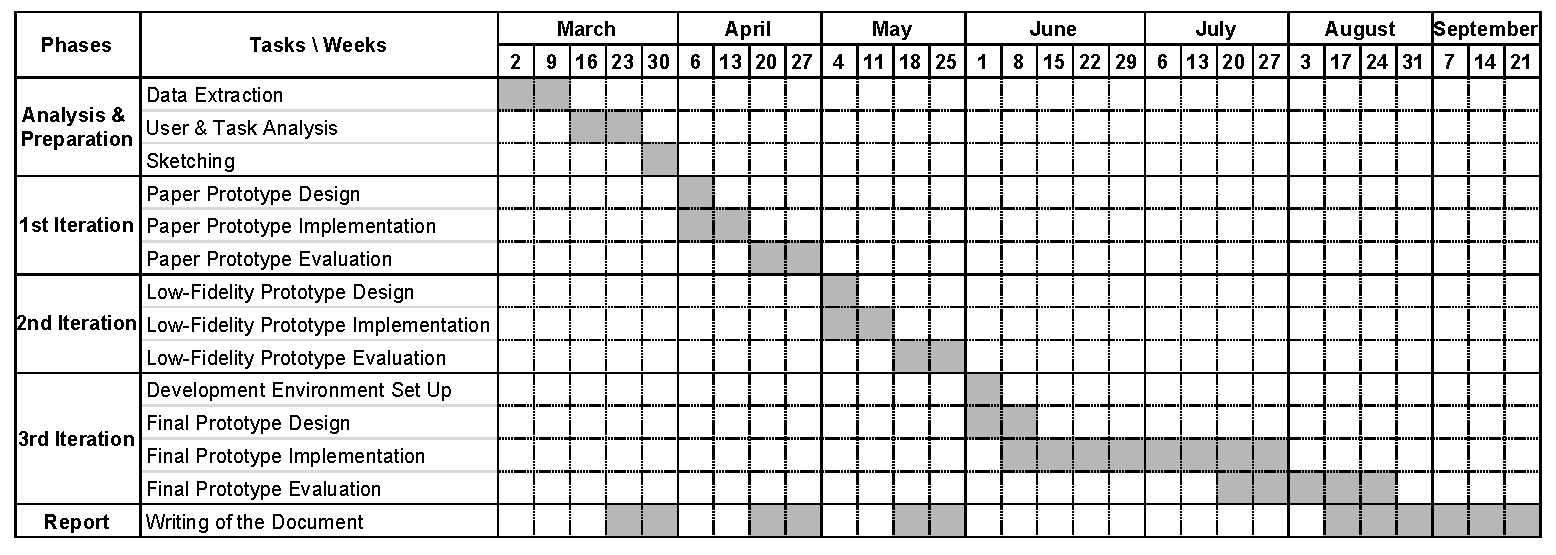
\includegraphics[width=1.0\textwidth]{workPlan}
	\caption{Task Scheduling throughout the weeks until the final of the project.}
	\label{fig:work_plan}
\end{figure}



